\chapter{Wyniki}\label{chapter:wyniki}

W ramach poniższego rozdziału przedstawiono wyniki badania, które będą kluczem w odpowiedzi na postawione w pracy pytania badawcze.
Rozdział obejmuje wyniki testów wydajnościowych funkcji oraz analizę wpływu metod optymalizacji na kryteria związane z procesem rozwoju oprogramowania.
W obrębie tej części pracy została zawarta obiektywna analiza wyników, co posłuży w następnym rozdziale do przedstawienia wniosków na ich bazie.

\section{Ciepły start}\label{chapter:results_warm_start}

Pierwszym kryterium badanym w testach wydajnościowych był czas działania funkcji podczas ciepłych startów.
Oznacza to sytuację, gdy funkcja była wywołana w momencie, gdy aktywna była jedna z instancji funkcji.
Powoduje to, że nie jest wymagana inicjalizacja usługi, a kod rozpoczyna działanie bezpośrednio po wywołaniu.
W badaniu każda funkcja została wywołana stukrotnie, a wyniki zostały zagregowane.
Średni czas wykonania w zależności od metody i rozmiaru pamięci został przedstawiony na Rysunku \ref{fig:avg_warm_start}.
Dokładne wartości badanych parametrów (czas średni, mediana, odchylenie standardowe) i różnice względem funkcji bazowej (Java JVM) zostały zaprezentowane w Tabeli \ref{table:warm_start_comparison}.

\begin{figure}[h]
    \centering
    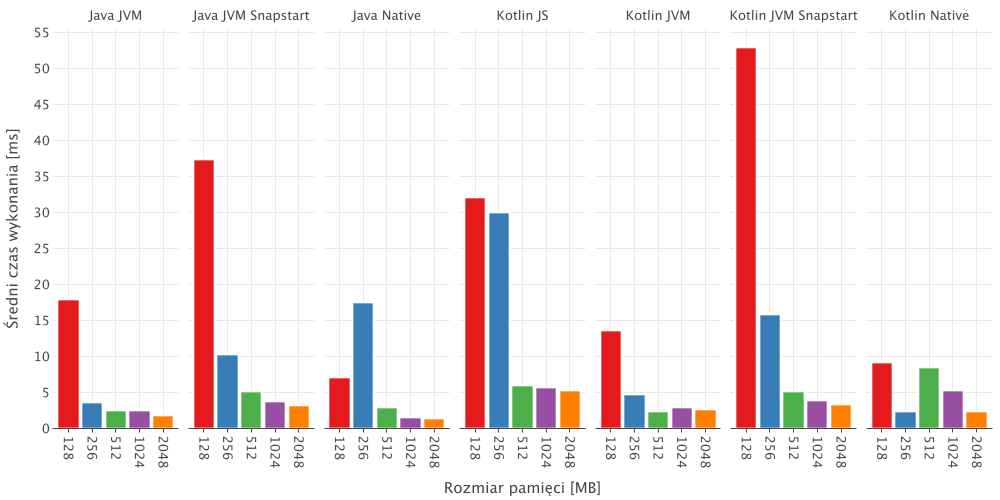
\includegraphics[width=0.95\textwidth]{charts/results/avg-warm-start.png}
    \caption{Średni czas wykonywania funkcji (ciepły start) z użyciem wybranych metod w zależności od rozmiaru pamięci [źródło: opracowanie własne]}
    \label{fig:avg_warm_start}
\end{figure}

Dla każdego z badanych rodzajów funkcji widoczne jest znaczne zróżnicowanie czasu wykonania w zależności od rozmiaru pamięci.
Sama skuteczność metod w poprawie wydajności różni się także ze względu na pamięć funkcji.
Pierwsza metoda, czyli usługa SnapStart, nie przyniosła poprawy czasu wykonania w żadnej z badanych wielkości pamięci.
Zastosowanie obrazów natywnych GraalVM pozwala na zmniejszenie czasu w niektórych rozmiarach pamięci: 128 MB, 1024 MB oraz 2048 MB.
Podobnie zachowuje się funkcja napisana w Kotlinie, działające w ramach JVM: tutaj poprawa jest widoczna dla pamięci 128 MB i 512 MB.

Funkcja działające w oparciu o kod JavaScript, stworzony poprzez translację Kotlin/JS, niesie negatywny wpływ na czas wykonania.
Metoda ta nie przyniosła poprawy w żadnym z badanych rozmiarów pamięci, przy czym w małych rozmiarach (128 MB, 256 MB) wpłynęła znacznie negatywnie na wydajność.
Dodatkowo, nie widać znacznej poprawy efektywności wraz z wzrostem rozmiaru pamięci z 512 MB do 2048 MB. 
Ciekawa zależność widoczna jest w przypadku funkcji Kotlin/Native, która wskazuje wykazuje poprawę czasu działania dla małych wielkości pamięci (128 MB i 256 MB).
Szczególna poprawa widoczna jest dla rozmiaru 256 MB, gdzie metoda ta osiągnęła niższe czasy wykonania niż funkcja Java JVM dla większych wielkości pamięci (512-2048 MB).

\begin{table}[htbp]
\centering
\caption{Porównanie średnich, median oraz odchyleń standardowych czasów działania funkcji podczas ciepłego startu względem funkcji bazowej (Java JVM) [źródło: opracowanie własne]}
\small
\begin{tabular}{|>{\centering\arraybackslash}m{2cm}|l|p{1.5cm}|p{1.5cm}|p{1.5cm}|p{1.5cm}|p{1.5cm}|}
\toprule
Rozmiar pamięci [MB] & Metoda & Średnia [ms] & Zmiana średniej & Mediana [ms] & Zmiana mediany & Odch. stand. \\
\midrule
\multirow{7}{*}{128} & Java JVM & 17.89 & \mbox{0\%} & 14.55 & \mbox{0\%} & 14.02 \\
 & Java GraalVM & 7.09 & \mbox{-60\%} & 1.13 & \mbox{-92\%} & 29.43 \\
 & Java JVM + SnapStart & 37.36 & \mbox{+109\%} & 35.86 & \mbox{+146\%} & 18.88 \\
 & Kotlin JVM & 13.56 & \mbox{-24\%} & 10.32 & \mbox{-29\%} & 19.70 \\
 & Kotlin JVM + SnapStart & 52.92 & \mbox{+196\%} & 44.69 & \mbox{+207\%} & 28.23 \\
 & Kotlin/JS & 32.15 & \mbox{+80\%} & 2.56 & \mbox{-82\%} & 63.63 \\
 & Kotlin/Native & 9.19 & \mbox{-49\%} & 7.08 & \mbox{-51\%} & 7.90 \\
\midrule
\multirow{7}{*}{256} & Java JVM & 3.66 & \mbox{0\%} & 2.16 & \mbox{0\%} & 4.59 \\
 & Java GraalVM & 17.48 & \mbox{+378\%} & 1.25 & \mbox{-42\%} & 24.41 \\
 & Java JVM + SnapStart & 10.31 & \mbox{+182\%} & 11.95 & \mbox{+453\%} & 7.45 \\
 & Kotlin JVM & 4.70 & \mbox{+29\%} & 2.13 & \mbox{-1\%} & 5.80 \\
 & Kotlin JVM + SnapStart & 15.87 & \mbox{+334\%} & 13.41 & \mbox{+521\%} & 12.12 \\
 & Kotlin/JS & 29.98 & \mbox{+720\%} & 10.24 & \mbox{+374\%} & 43.71 \\
 & Kotlin/Native & 2.37 & \mbox{-35\%} & 2.06 & \mbox{-5\%} & 1.70 \\
\midrule
\multirow{7}{*}{512} & Java JVM & 2.56 & \mbox{0\%} & 2.37 & \mbox{0\%} & 0.62 \\
 & Java GraalVM & 2.87 & \mbox{+12\%} & 1.30 & \mbox{-45\%} & 6.34 \\
 & Java JVM + SnapStart & 5.15 & \mbox{+101\%} & 2.86 & \mbox{+21\%} & 4.88 \\
 & Kotlin JVM & 2.41 & \mbox{-6\%} & 2.03 & \mbox{-14\%} & 1.24 \\
 & Kotlin JVM + SnapStart & 5.13 & \mbox{+101\%} & 2.94 & \mbox{+24\%} & 5.26 \\
 & Kotlin/JS & 5.94 & \mbox{+132\%} & 1.97 & \mbox{-17\%} & 11.96 \\
 & Kotlin/Native & 8.45 & \mbox{+231\%} & 6.80 & \mbox{+187\%} & 6.35 \\
\midrule
\multirow{7}{*}{1024} & Java JVM & 2.48 & \mbox{0\%} & 2.42 & \mbox{0\%} & 0.27 \\
 & Java GraalVM & 1.48 & \mbox{-40\%} & 1.01 & \mbox{-58\%} & 2.44 \\
 & Java JVM + SnapStart & 3.74 & \mbox{+51\%} & 2.92 & \mbox{+21\%} & 2.30 \\
 & Kotlin JVM & 2.89 & \mbox{+17\%} & 2.75 & \mbox{+14\%} & 0.95 \\
 & Kotlin JVM + SnapStart & 3.89 & \mbox{+57\%} & 3.09 & \mbox{+28\%} & 1.80 \\
 & Kotlin/JS & 5.66 & \mbox{+129\%} & 3.04 & \mbox{+26\%} & 6.65 \\
 & Kotlin/Native & 5.31 & \mbox{+114\%} & 6.57 & \mbox{+171\%} & 2.13 \\
\midrule
\multirow{7}{*}{2048} & Java JVM & 1.81 & \mbox{0\%} & 1.44 & \mbox{0\%} & 0.70 \\
 & Java GraalVM & 1.40 & \mbox{-23\%} & 1.07 & \mbox{-26\%} & 1.75 \\
 & Java JVM + SnapStart & 3.26 & \mbox{+80\%} & 2.80 & \mbox{+94\%} & 1.01 \\
 & Kotlin JVM & 2.62 & \mbox{+44\%} & 2.12 & \mbox{+47\%} & 1.19 \\
 & Kotlin JVM + SnapStart & 3.40 & \mbox{+88\%} & 2.88 & \mbox{+100\%} & 1.63 \\
 & Kotlin/JS & 5.26 & \mbox{+190\%} & 4.02 & \mbox{+179\%} & 3.76 \\
 & Kotlin/Native & 2.36 & \mbox{+30\%} & 2.24 & \mbox{+56\%} & 0.38 \\
\bottomrule
\end{tabular}
\label{table:warm_start_comparison}
\end{table}

Na Rysunkach \ref{fig:warm_start_256} oraz \ref{fig:warm_start_1024} przedstawiono wykresy pudełkowe z czasami wykonania funkcji dla rozmiarów pamięci 256 MB i 1024 MB.
Funkcje oparte wyłącznie o maszynę wirtualną wykazały najmniej zróżnicowane wyniki.
Aktywacja funkcji SnapStart znacząco obniżyła stabilność czasów odpowiedzi, podobnie jak Kotlin/JS.
Warte zwrócenia uwagi są jednak funkcje natywne. 
Obrazy GraalVM wykazują jednolite wyniki, oprócz pamięci 256 MB, gdzie czas wykonania znacząco różnił się w poszczególnych wywołaniach.
Podobna zależność występuje dla funkcji Kotlin/Native, które osiągają niestabilne wyniki dla rozmiarów pamięci 512 MB oraz 1024 MB.

% --- Row 1: 256 MB and 1024 MB charts ---
\begin{figure}[h]
    \centering % Center the minipages on the line
    \begin{minipage}[t]{0.48\textwidth} % [t] for top alignment
        \centering % Center content within this minipage
        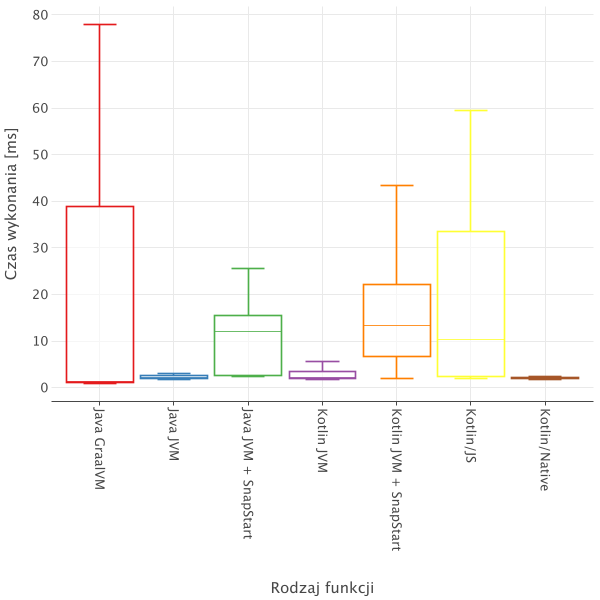
\includegraphics[width=\linewidth]{charts/results/warm-start-boxplot-256.png}
        \captionof{figure}{Czas wykonania funkcji (ciepły start, 256 MB) [źródło: opracowanie własne]}
        \label{fig:warm_start_256} % Unique label for this figure
    \end{minipage}% <--- % is important
    \hfill % Space between minipages
    \begin{minipage}[t]{0.48\textwidth}
        \centering
        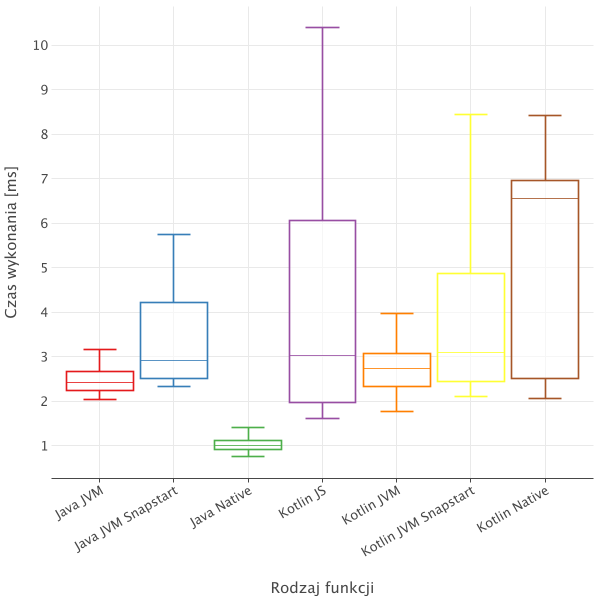
\includegraphics[width=\linewidth]{charts/results/warm-start-boxplot-1024.png}
        \captionof{figure}{Czas wykonania funkcji (ciepły start, 1024 MB) [źródło: opracowanie własne]}
        \label{fig:warm_start_1024} % Unique label
    \end{minipage}
    % No overall \caption for this outer figure environment, as it's just for layout.
\end{figure}

\begin{table}[H]
    \centering
    \caption{Wyniki testu Kruskal-Wallis dla wyników pomiaru czasu działania funkcji podczas ciepłych startów [źródło: opracowanie własne]}
    \begin{tabular}{|c|c|}
    \hline
    \textbf{Wielkość pamięci [MB]} & \textbf{Wartość p} \\
    \hline
    128 & $6.46 \times 10^{-38}$ \\
    \hline
    256 & $1.65 \times 10^{-18}$ \\
    \hline
    512 & $9.37 \times 10^{-43}$ \\
    \hline
    1024 & $3.62 \times 10^{-72}$ \\
    \hline
    2048 & $1.69 \times 10^{-72}$ \\
    \hline
    \end{tabular}
    \label{table:kruskal_wallis_test_warm_starts}
\end{table}

\begin{table}[H]
    \caption{Porównanie czasów działania funkcji podczas ciepłych startów poprzez wartość p testu Dunn (\textbf{istotne różnice pogrubione}) [źródło: opracowanie własne]}
    \centering
    \footnotesize
    \begin{tabular}{|p{3cm}|>{\raggedright\arraybackslash}p{3cm}|>{\raggedright\arraybackslash}p{1.5cm}|>{\raggedright\arraybackslash}p{1.5cm}|>{\raggedright\arraybackslash}p{1.5cm}|>{\raggedright\arraybackslash}p{1.5cm}|>{\raggedright\arraybackslash}p{1.5cm}|}
    \hline
    \multirow{2}{*}{\textbf{Pierwsza funkcja}} & \multirow{2}{*}{\textbf{Druga funkcja}} & \multicolumn{5}{c|}{\textbf{Wielkość pamięci [MB]}} \\
    \cline{3-7}
    & & \textbf{128} & \textbf{256} & \textbf{512} & \textbf{1024} & \textbf{2048} \\
    \hline
    \multirow{6}{*}{Java GraalVM} & Java JVM & $\bm{5.44 \times 10^{-16}}$ & 0.7368 & $\bm{5.51 \times 10^{-11}}$ & $\bm{1.93 \times 10^{-9}}$ & $\bm{2.08 \times 10^{-16}}$ \\ 
    \cline{2-7}
    & Java JVM + SnapStart & $\bm{1.29 \times 10^{-25}}$ & $\bm{4.78 \times 10^{-8}}$ & $\bm{1.48 \times 10^{-19}}$ & $\bm{2.65 \times 10^{-21}}$ & $\bm{2.52 \times 10^{-34}}$ \\
    \cline{2-7}
    & Kotlin JVM & $\bm{9.37 \times 10^{-10}}$ & 0.6159 & $\bm{9.01 \times 10^{-5}}$ & $\bm{4.54 \times 10^{-32}}$ & $\bm{5.90 \times 10^{-19}}$ \\
    \cline{2-7}
    & Kotlin JVM + SnapStart & $\bm{4.27 \times 10^{-32}}$ & $\bm{5.80 \times 10^{-10}}$ & $\bm{2.98 \times 10^{-18}}$ & $\bm{9.73 \times 10^{-21}}$ & $\bm{8.19 \times 10^{-33}}$ \\
    \cline{2-7}
    & Kotlin/JS & $\bm{6.55 \times 10^{-15}}$ & $\bm{3.89 \times 10^{-10}}$ & $\bm{3.05 \times 10^{-9}}$ & $\bm{3.32 \times 10^{-20}}$ & $\bm{8.88 \times 10^{-39}}$ \\
    \cline{2-7}
    & Kotlin/Native & $\bm{9.37 \times 10^{-10}}$ & 1.0000 & $\bm{3.86 \times 10^{-34}}$ & $\bm{1.11 \times 10^{-66}}$ & $\bm{1.37 \times 10^{-19}}$ \\
    \hline
    \multirow{5}{*}{Java JVM} & Java JVM + SnapStart & 0.0740 & \textbf{0.0042} & 0.0835 & \textbf{0.0359} & $\bm{1.89 \times 10^{-10}}$ \\
    \cline{2-7}
    & Kotlin JVM & 0.3281 & 1.0000 & 0.0893 & 0.4362 & \textbf{0.0153} \\
    \cline{2-7}
    & Kotlin JVM + SnapStart & \textbf{0.0011} & $\bm{5.69 \times 10^{-4}}$ & 0.1263 & \textbf{0.0329} & $\bm{2.38 \times 10^{-9}}$ \\
    \cline{2-7}
    & Kotlin/JS & 0.1164 & $\bm{6.92 \times 10^{-4}}$ & 0.1195 & 0.1252 & $\bm{8.36 \times 10^{-12}}$ \\
    \cline{2-7}
    & Kotlin/Native & 0.3281 & 1.0000 & $\bm{5.70 \times 10^{-4}}$ & $\bm{5.29 \times 10^{-8}}$ & \textbf{0.0104} \\
    \hline
    \multirow{4}{\linewidth}{Java JVM + SnapStart} & Kotlin JVM & $\bm{9.08 \times 10^{-5}}$ & \textbf{0.0057} & $\bm{8.12 \times 10^{-6}}$ & 0.4362 & \textbf{0.0153} \\
    \cline{2-7}
    & Kotlin JVM + SnapStart & 0.9682 & 1.0000 & 1.0000 & 1.0000 & 1.0000 \\
    \cline{2-7}
    & Kotlin/JS & $\bm{7.12 \times 10^{-7}}$ & 1.0000 & $\bm{1.09 \times 10^{-6}}$ & 1.0000 & 1.0000 \\
    \cline{2-7}
    & Kotlin/Native & $\bm{9.08 \times 10^{-5}}$ & $\bm{1.06 \times 10^{-4}}$ & 1.0000 & 0.3242 & \textbf{0.0180} \\
    \hline
    \multirow{3}{*}{Kotlin JVM} & Kotlin JVM + SnapStart & $\bm{1.59 \times 10^{-7}}$ & $\bm{7.84 \times 10^{-4}}$ & $\bm{3.48 \times 10^{-5}}$ & 0.4362 & \textbf{0.0349} \\
    \cline{2-7}
    & Kotlin/JS & 1.0000 & $\bm{9.48 \times 10^{-4}}$ & 1.0000 & 0.8655 & \textbf{0.0106} \\
    \cline{2-7}
    & Kotlin/Native & 1.0000 & 1.0000 & $\bm{5.51 \times 10^{-11}}$ & $\bm{5.91 \times 10^{-8}}$ & 1.0000 \\
    \hline
    \multirow{2}{\linewidth}{Kotlin JVM + SnapStart} & Kotlin/JS & $\bm{5.86 \times 10^{-11}}$ & 1.0000 & $\bm{8.12 \times 10^{-6}}$ & 1.0000 & 1.0000 \\
    \cline{2-7}
    & Kotlin/Native & $\bm{1.59 \times 10^{-7}}$ & $\bm{7.13 \times 10^{-6}}$ & 0.8982 & 0.4362 & \textbf{0.0427} \\
    \hline
    Kotlin/JS & Kotlin/Native & 1.0000 & $\bm{8.07 \times 10^{-6}}$ & $\bm{2.04 \times 10^{-17}}$ & \textbf{0.0466} & \textbf{0.0153} \\
    \hline
    \end{tabular}
    \label{table:dunn_results_warm_starts}
\end{table}


\newpage
\section{Zimny start}\label{chapter:results_cold_start}

Drugim badanym kryterium jest czas działania funkcji podczas zimnych startów, które wymagają odpowiedniej inicjaliacji funkcji.
Z reguły są one dłuższe niż ciepłe starty, co może szczególnie wpłynąć na ogólną wydajność \cite{9284261}\cite{8605777}.
Średni czas działania funkcji został przedstawiony na Rysunkach \ref{fig:avg_cold_start_128_256}, \ref{fig:avg_cold_start_512_2045} oraz w Tabeli \ref{table:cold_start_comparison}.

\begin{figure}[!h]
    \centering
    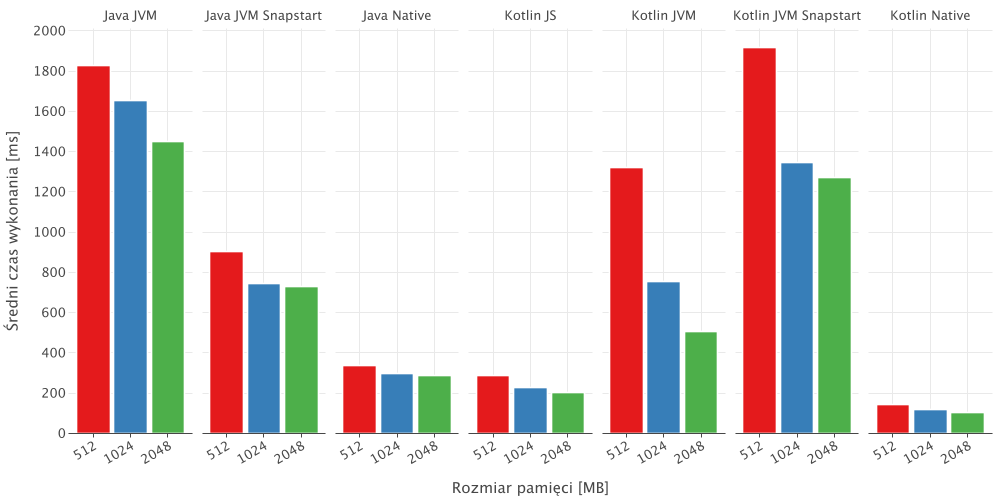
\includegraphics[width=0.95\textwidth]{charts/results/avg-cold-start-512-2048.png}
    \caption{Średni czas wykonywania funkcji (zimny start) dla rozmiarów pamięci: 512 MB, 1024 MB, 2048 MB  [źródło: opracowanie własne]}
    \label{fig:avg_cold_start_512_2045}
\end{figure}

Wpływ aktywacji usługi SnapStart jest różny w zależności od języka oprogramowania.
Dla Javy, usługa ta pozwoliła na poprawę czasu działania funkcji, w szczególności dla większych rozmiarów pamięci.
W przypadku języka Kotlin, jej aktywacja wpłynęła negatywnie na wydajność, wydłużając czas procesowania.
Samo użycie Kotlina (działającego w oparciu o JVM) pozwoliło na przyspieszenie obliczeń dla większych rozmiarów pamięci (512-2048 MB).

Znaczna poprawa wydajności została osiągnięte dla funkcji opartych o GraalVM oraz Kotlin/JS.
Obie metody uzyskały podobne wyniki, przy czym funkcja natywna GraalVM osiągnęła poprawę w przypadku rozmiarów pamięci 128 MB i 256 MB.
Dla wielkości 512-2048 MB, Kotlin/JS osiągnął niższe czasy działania niż funkcja GraalVM.
Niezależnie od rozmiaru pamięci najkrótszy czas działania w przypadku zimnego startu osiągnęły funkcje oparte o technologię Kotlin/Native.
Metoda ta pozwoliła także na osiągnięcie wyników o podobnej stabilności jak pozostałe funkcje, co zostało przedstawione na Rysunkach \ref{fig:warm_start_256} i \ref{fig:warm_start_1024}.
Mocno zróżnicowane wyniki zostały osiągnięte przez funkcję Kotlin z aktywowaną funkcją SnapStart.

\begin{table}[h]
    \caption{Porównanie średnich czasów działania funkcji podczas zimnego startu względem funkcji bazowej [źródło: opracowanie własne]}
    \centering
    % Modified column definitions for left alignment
    \begin{tabular}{|>{\raggedright\arraybackslash}p{3.5cm}|>{\raggedright\arraybackslash}p{1.8cm}|>{\raggedright\arraybackslash}p{1.8cm}|>{\raggedright\arraybackslash}p{1.8cm}|>{\raggedright\arraybackslash}p{1.8cm}|>{\raggedright\arraybackslash}p{1.8cm}|}
    \hline
    % Header: First cell's \makecell changed to [l] for left alignment
    \multirow{2}{*}{\makecell[l]{\textbf{Rodzaj funkcji} \\ \scriptsize{\textit{Czas [ms] (\% różnicy)}}}} & \multicolumn{5}{c|}{\textbf{Rozmiar pamięci [MB]}} \\ % Kept multicolumn centered, change 'c' to 'l' if left-align needed
    \cline{2-6} 
    & \textbf{128} & \textbf{256} & \textbf{512} & \textbf{1024} & \textbf{2048} \\
    \hline
    Java JVM & 2726 & 2165 & 1827 & 1652 & 1450 \\
    \hline
    Java JVM +~SnapStart & 2466 \mbox{(-10\%)} & 1287 \mbox{(-41\%)} & 901 \mbox{(-51\%)} & 745 \mbox{(-55\%)} & 731 \mbox{(-50\%)} \\
    \hline
    Java GraalVM & 596 \mbox{(-78\%)} & 417 \mbox{(-81\%)} & 335 \mbox{(-82\%)} & 299 \mbox{(-82\%)} & 287 \mbox{(-80\%)} \\
    \hline
    Kotlin JVM & 4927 \mbox{(81\%)} & 2426 \mbox{(12\%)} & 1320 \mbox{(-28\%)} & 754 \mbox{(-54\%)} & 504 \mbox{(-65\%)} \\
    \hline
    Kotlin JVM +~SnapStart & 5853 \mbox{(115\%)} & 3185 \mbox{(47\%)} & 1915 \mbox{(5\%)} & 1347 \mbox{(-18\%)} & 1272 \mbox{(-12\%)} \\
    \hline
    Kotlin/JS & 679 \mbox{(-75\%)} & 424 \mbox{(-80\%)} & 287 \mbox{(-84\%)} & 228 \mbox{(-86\%)} & 201 \mbox{(-86\%)} \\
    \hline
    Kotlin/Native & 328 \mbox{(-88\%)} & 204 \mbox{(-91\%)} & 143 \mbox{(-92\%)} & 119 \mbox{(-93\%)} & 105 \mbox{(-93\%)} \\
    \hline
    \end{tabular}
    \label{table:cold_start_comparison}
\end{table}

\begin{figure}[p] % Use [p] to suggest a float page. Or [!htbp] for more flexibility.
    \centering

    % --- First graphical element ---
    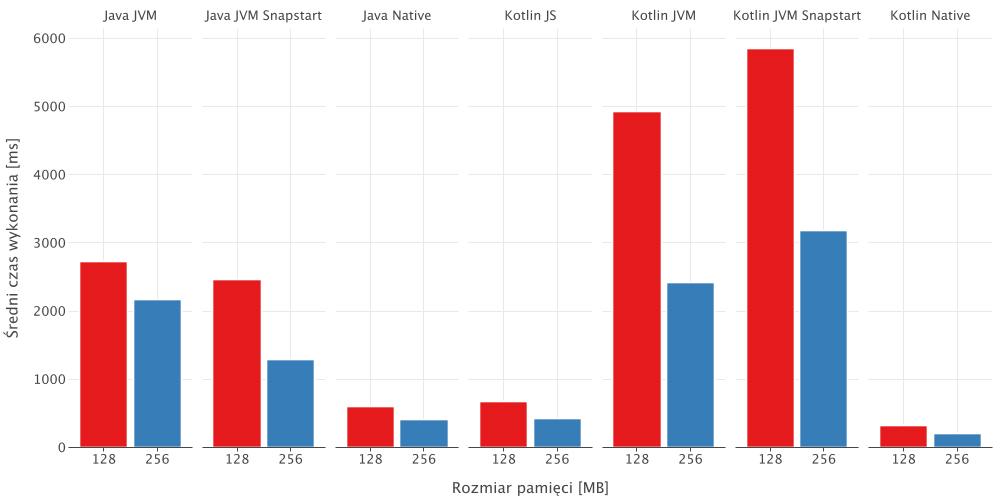
\includegraphics[width=0.95\textwidth]{charts/results/avg-cold-start-128-256.png}
    \caption{Średni czas wykonywania funkcji (zimny start) dla rozmiarów pamięci: 128 MB, 256 MB  [źródło: opracowanie własne]}
    \label{fig:avg_cold_start_128_256}

    \vspace{2em} % Optional: Add some vertical space between the distinct parts within this single figure

    % --- Second graphical element (with minipages) ---
    % Note: No new \begin{figure} here. This is part of the same float.
    \begin{minipage}[t]{0.48\textwidth}
        \centering
        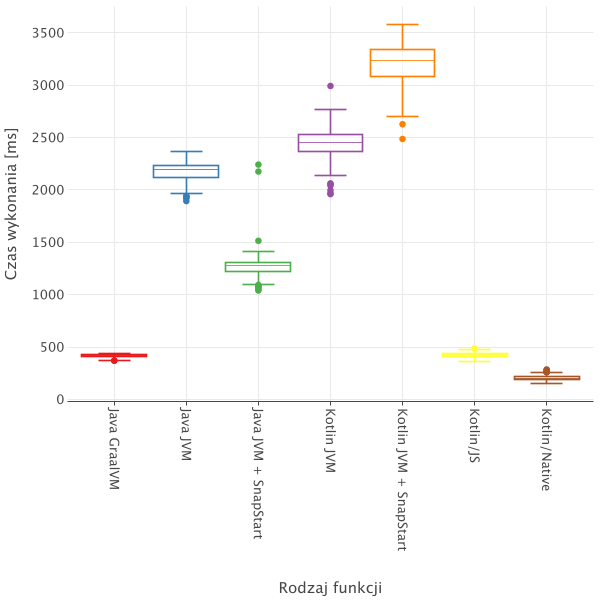
\includegraphics[width=\linewidth]{charts/results/cold-start-boxplot-256.png}
        \captionof{figure}{Czas wykonania funkcji (zimny start, 256 MB) [źródło: opracowanie własne]} % \captionof requires the 'caption' or 'capt-of' package
        \label{fig:cold_start_128}
    \end{minipage}% <--- % is important to prevent extra horizontal space
    \hfill % Creates flexible space between the minipages
    \begin{minipage}[t]{0.48\textwidth}
        \centering
        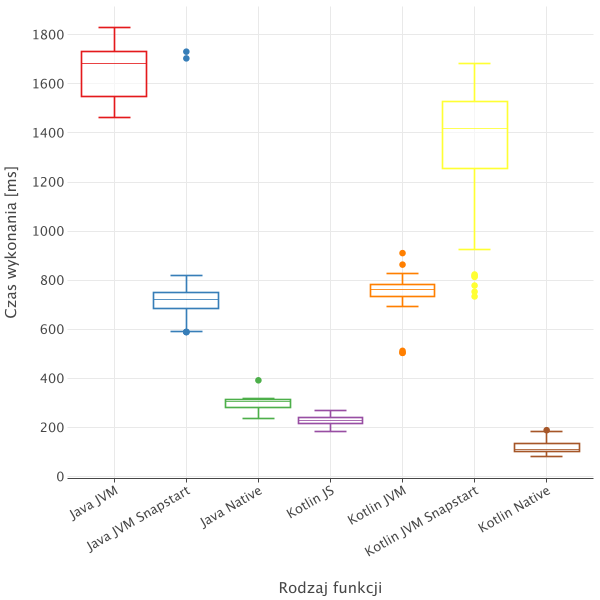
\includegraphics[width=\linewidth]{charts/results/cold-start-boxplot-1024.png}
        \captionof{figure}{Czas wykonania funkcji (zimny start, 1024 MB) [źródło: opracowanie własne]}
        \label{fig:cold_start_256}
    \end{minipage}
    % If this combined figure needs an overall caption, you could add another \caption{} here.
    % If the first caption serves as the overall caption, then this is fine.
\end{figure}


\newpage
\section{Współczynnik wydajności funkcji}\label{chapter:results_wwf}

Kolejnym badanym kryterium jest współczynnik wydajności funkcji (WWF), opisany w Rozdziale \ref{chapter:cel_i_metodologia_badan}.
Pozwala on na jednoczesną analizę zarówno ciepłych, jak i zimnych startów, a wyższe wartości WWF oznaczają wyższą wydajność funkcji.
Wartości WWF zostały obliczone na bazie średnich czasów wykonania podczas zimnych i ciepłych startów.
W ramach obliczeń przyjęto wagi: 0,975 dla ciepłych startów oraz 0,025 dla zimnych startów.
Wyniki dla poszczególnych metod i rozmiarów pamięci zostały przedstawione na Rysunku \ref{fig:avg_wwf}.

\begin{figure}[h]
    \centering
    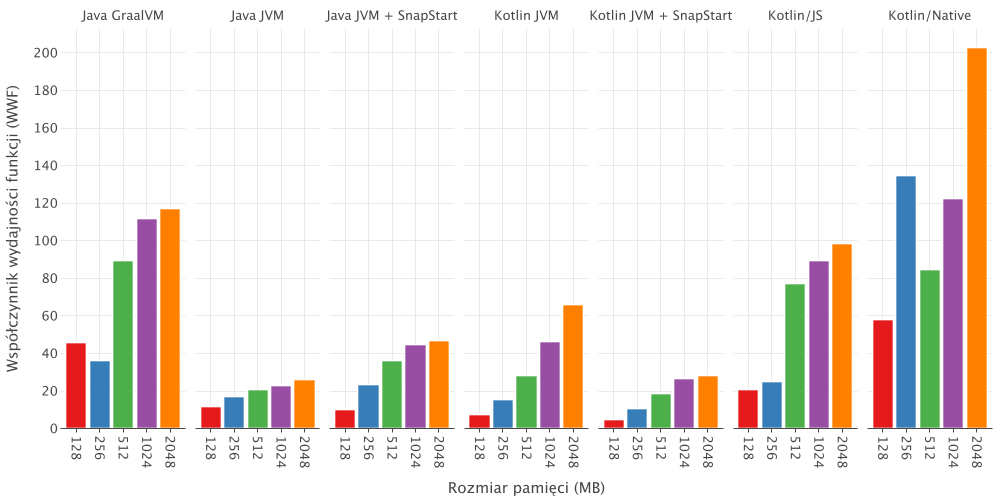
\includegraphics[width=0.95\textwidth]{charts/results/wwf.png}
    \caption{Współczynnik wydajności funkcji w zależności od rozmiaru pamięci [źródło: opracowanie własne]}
    \label{fig:avg_wwf}
\end{figure}

Dla funkcji Java opartej o JVM, wartość współczynnika rośnie wraz z wzrostem pamięci.
Podobny trend występuje dla funkcji Kotlin JVM, gdzie jednak wzrost ten jest bardziej dynamiczny.
Dla małych rozmiarów pamięci funkcje Kotlin charakteryzują się mniejszą wydajnością, jednak zmienia się to dla wyższych wartości pamięci (od 512 MB wzyż).
Skuteczność użycia usługi SnapStart zależy od użytego języka programowania.
W przypadku Javy, wydajność poprawiła się dla wszystkich rozmiarów pamięci oprócz 128 MB. 
Dla Kotlina wydajność pogorszyła się (w porównaniu z funkcjami Kotlin JVM) dla wszystkich rozmiarów pamięci, gdzie wraz z zwiększaniem wielkości pamięci różnica pogłębia się.

Znaczną poprawę wydajności dla wszystkich rozmiarów pamięci zauważono w funkcjach Java GraalVM, Kotlin/JS oraz Kotlin/Native.
W przypadku dwóch pierwszych widoczny jest znaczny wzrost wartości WWF dla rozmiarów pamięci niemniejszych niż 512 MB.
Dla tych rozmiarów pamięci obie te funkcje wykazują podobną wydajność, jednak z przewagą dla funkcji Java GraalVM.
Przewaga ta jest znacznie większa dla mniejszych pojemności pamięci (128 MB i 256 MB).
Najlepszą wartością współczynnika charakteryzuje się jednak użycie Kotlin/Native, gdzie współczynnik osiągnął najlepsze wartość dla wszystkich rozmiarów pamięci oprócz 512 MB.
Jednak dla pamięci 512 MB, wartość WWF jest około 4\% niższa dla Kotlin/Native niż Java GraalVM.
Warte zwrócenia uwagi są jednak badania przeprowadzone dla rozmiarów pamięci 256 MB i 2048 MB, gdzie Kotlin/Native osiągnął znacznie wyższe wartości WWF niż pozostałe funkcje.
W porównaniu z Java GraalVM, czyli drugą najbardziej skuteczną metodą, wartości są wyższe o około 275\% i 74\%.


\section{Koszt funkcji}\label{chapter:results_cost}

Miarą, która wynika bezpośrednio z czasu działania funkcji oraz rozmiaru jej pamięci jest koszt jej działania.
W ramach badania został on obliczony na bazie średnich czasów procesowania funkcji, co zostało opisane w Rodziale \ref{chapter:cel_i_metodyka_badan}.
W obliczeniach przyjęto 500 wywołań funkcji na sekundę oraz koszt 0.0000166667 USD za GB-sekundę \cite{awsLambdaPricing}.
Wyniki dla poszczególnych metod i rozmiarów pamięci zostały przedstawione na Rysunku \ref{fig:avg_costs}.

\begin{figure}[h]
    \centering
    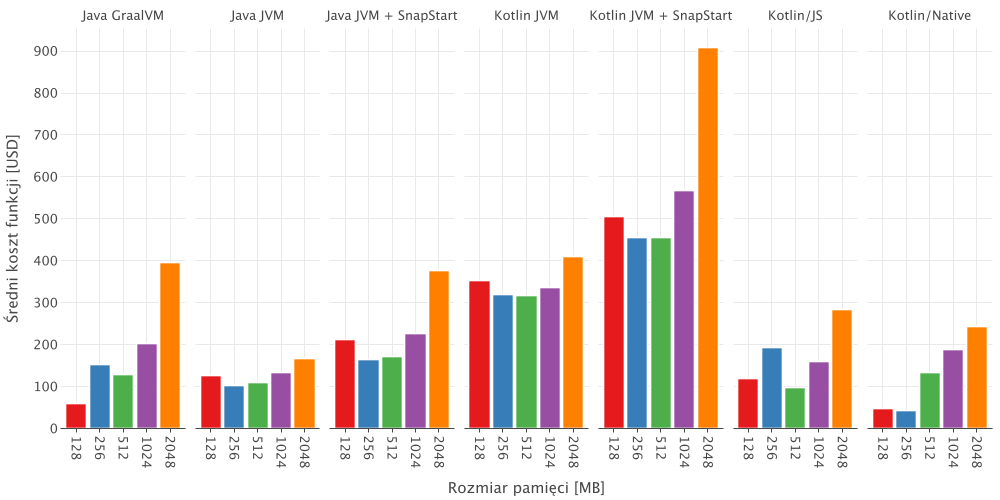
\includegraphics[width=0.95\textwidth]{charts/results/average-cost.png}
    \caption{Średni koszt funkcji w zależności od rozmiaru pamięci [źródło: opracowanie własne]}
    \label{fig:avg_costs}
\end{figure}

Analizując cztery funkcje oparte o JVM można zauważyć, że koszt jest najniższy dla pamięci 256 MB lub 512 MB.
Interesującym faktem jest, że rozmiaru 128 MB koszt działania jest wyższy, co przeczy oczekiwaniom, że koszty maleją wraz z spadkiem wielkości pamięci, niezależnie od jej wartości.
Dla funkcji bez aktywowanej usługi SnapStart koszt dla pamięci 128 MB jest nawet wyższy niż dla wielkości 512 MB.
Podczas aktywnej usługi SnapStart, badane funkcje wykazują znaczny wzrost średnich kosztów wraz z wzrostem pamięci z 1024 MB do 2048 MB.
Sama metoda SnapStart wpływa jednak negatywnie na koszt działania.
Znaczne oddziaływanie rozmiaru pamięci na koszt funkcji jest istotnie widoczny dla Kotlin/JS.
Koszt jest znacznie zróżnicowany, jednak dla pewnych przypadków (pamięć 128 MB i 512 MB) pozostaje on niższy niż w przypadku funkcji Java JVM.

Obie z badanych funkcji natywnych (Java GraalVM, Kotlin/Native) wykazują wzrost kosztów wraz z wzrostem rozmiaru pamięci.
Dla każdego rozmiaru pamięci oprócz 128 MB, koszty funkcji Java GraalVM są wyższe niż dla analogicznej funkcji Java JVM.
Widoczny jest także znaczny wzrost kosztów dla pamięci 2048 MB, podobnie jak w przypadku usługi SnapStart.
W przypadku użycia Kotlin/Native i pamięci 128 MB lub 256 MB możliwe jest osiągnięcie najniższych kosztów działanio (odpowiednio 48 i 43 USD).
Dla większych rozmiarów najlepsze wyniki zostały osiągnięte przez Kotlin/JS (rozmiary 512 MB) i Java JVM (rozmiary 1024 MB i 2048 MB).


\section{Wpływ na rozwój oprogramowania}\label{chapter:development-process}

Obszarem, który został także ujęty w badaniu jest wpływ poszczególnych metod na proces rozwoju oprogramowania.
Oceniono go z użyciem kryteriów, które zostały opisane w Rozdziale \ref{chapter:cel_i_metodyka_badan}.
W ramach rozdziału dokonano oceny metod, pod względem poszczególnych kryteriów.

\begin{figure}[h]
    \centering
    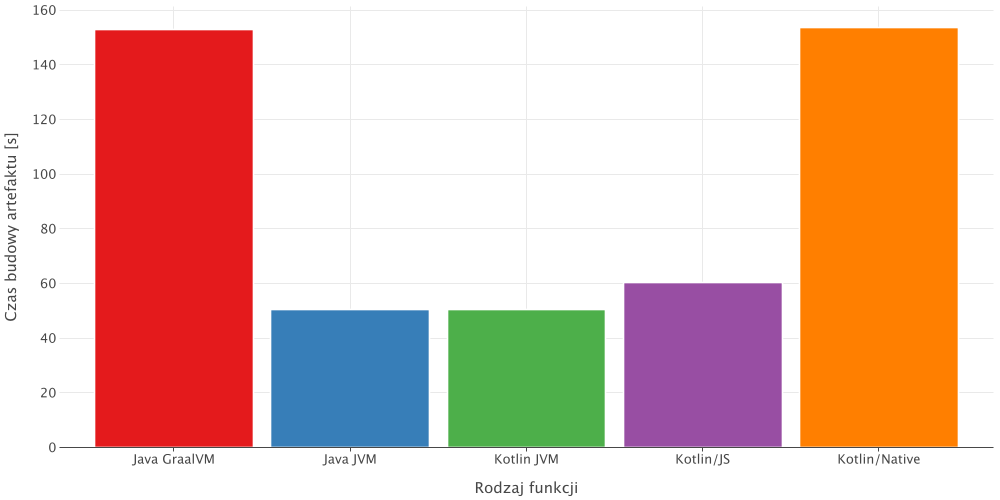
\includegraphics[width=0.95\textwidth]{charts/results/avg-build-times.png}
    \caption{Średni czas budowy artefaktu dla poszczególnych rodzajów funkcji [źródło: opracowanie własne]}
    \label{fig:avg_build_times}
\end{figure}

Średni czas budowy artefaktów został przedstawiony na Rysunku \ref{fig:avg_build_times}.
Funkcje z aktywną usługą SnapStart korzystają z artefaktów wytworzonych dla funkcji Java JVM i Kotlin JVM, dlatego nie zostały ujęte jako osobne rodzaje.
Czas tworzenia plików wdrożeniowych dla funkcji Java JVM i Kotlin JVM jest podobny, co wskazuje na nieznaczny wpływ Kotlina na ten proces.
W przypadku użycia Kotlin/JS translacja wymaga więcej czasu i widoczny jest jego wzrost o około 20\%.
Istotny jest jednak wpływ metod natywnych, gdzie wzrost wynosi już około 200\%.
Wyniki dla tych metod są podobne niezależnie od wybranego języka programowania (Javy lub Kotlina).

\begin{figure}[h]
    \centering
    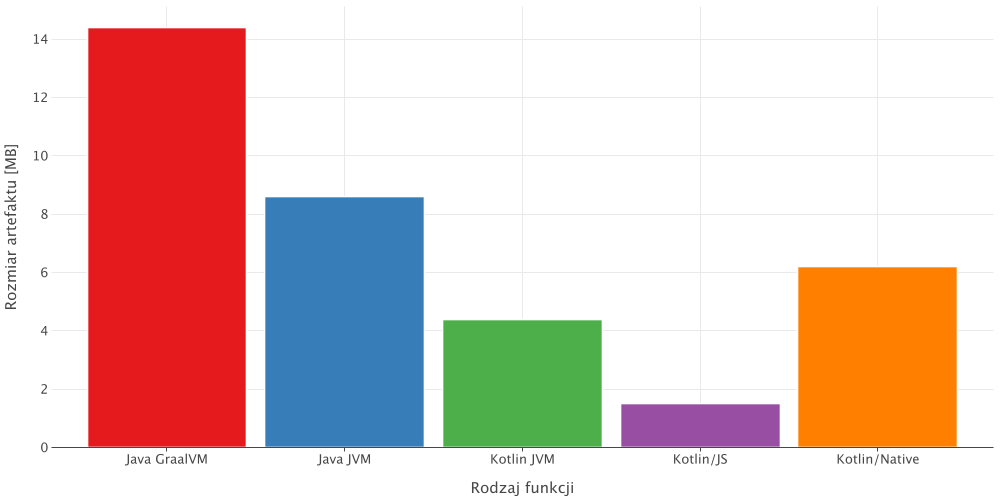
\includegraphics[width=0.95\textwidth]{charts/results/artifact-size.png}
    \caption{Wielkość artefaktu dla poszczególnych rodzajów funkcji [źródło: opracowanie własne]}
    \label{fig:artifact_size}
\end{figure}

Wielkość artefaktu dla poszczególnych rodzajów funkcji został przedstawiony na Rysunku \ref{fig:artifact_size}.
Dla tego kryterium, istotny wpływ ma wybrany język programowania.
Dla Javy wielkość plików jest większa, szczególnie dla obrazów natywnych GraalVM, gdzie osiątnięto rozmiar około 14 MB (około 67\% niż analogiczny plik JAR dla funkcji Java JVM).
Kotlin wykazuje się mniejszymi artefaktami, gdzie dla funkcji JVM rozmiar pliku JAR jest około 49\% mniejszy niż dla analogicznego artefaktu Java.
Translacja do języka JavaScript przyniosła bardzo pozytywne rezultaty gdzie osiągnięto najniższy rozmiar, około 1.5 MB.
Użycie kompilacji do binarnych plików natywnych z Kotlin/Native zwiększyło rozmiar artefaktu do około 6.2 MB, czyli około 41\% więcej niż plik JAR dla Kotlin JVM.
Metoda ta jednak pozwoliła na budowę o wiele mniejszego artefaktu niż analogiczna kompilacja z użyciem GraalVM.
Artefakt Kotlin/Native był w tym przypadku o 57\% mniejszy.

\begin{table}[h]
    \caption{Dostępność AWS SDK dla rodzajów funkcji [źródło: opracowanie własne]}
    \centering
    \begin{tabular}{|p{3cm}|p{3cm}|p{7cm}|} % Adjusted widths for demonstration
    \hline
    \textbf{Rodzaj funkcji} & \textbf{Dostępność AWS SDK} & \textbf{Komentarz} \\
    \hline
    Java JVM & Tak & Dedykowane AWS SDK dla Javy \cite{aws-sdk-java-v2}. \\
    \hline
    Kotlin JVM & Tak & Dedykowane AWS SDK dla Kotlina \cite{aws-sdk-kotlin}. \\
    \hline
    Java GraalVM & Tak & Wsparcie dla GraalVM poprzez AWS SDK dla Javy \cite{aws-sdk-java-v2}. \\
    \hline
    Kotlin/Native & Nie & AWS SDK dla Kotlina nie jest dostępne dla tej platformy. W momencie pisania pracy (maj 2025), wsparcie to jest w trakcie rozwoju \cite{aws-sdk-kotlin}. \\
    \hline
    Kotlin/JS & Tak & Poprzez użycie AWS SDK dla JavaScript \cite{aws-sdk-js-v3}. Nie jest jednak bezpośrednio zintegrowane z Kotlinem i użycie wymaga dodatkowych nakładów pracy. \\
    \hline
    \end{tabular}
    \label{table:aws_sdk_availability}
\end{table}

Dostępność bibliotek AWS SDK dla poszczególnych rodzajów funkcji została przedstawiona w Tabeli \ref{table:aws_sdk_availability}.
W przypadku funkcji Java JVM, Kotlin JVM oraz Java GraalVM dostępne są dedykowane biblioteki AWS SDK, co znacząco ułatwia integrację z usługami AWS. 
Sytuacja zmienia się w przypadku Kotlin/Native, dla którego AWS SDK nie jest jeszcze dostępne. 
Dla Kotlin/JS istnieje możliwość użycia AWS SDK dla JavaScript, jednak nie jest to rozwiązanie bezpośrednio zintegrowane z Kotlinem.
Wiąże się z koniecznością dodatkowych nakładów pracy i oraz utrzymywania dodatkowego kodu, co może znacząco wpłynąć na jakość rozwoju oprogramowania.


% TODO: wyniki wydajnościowe

% TODO: wyniki z PB3